\documentclass[10pt,letterpaper]{report}
\usepackage[utf8]{inputenc}
\usepackage[spanish]{babel}
\usepackage{amsmath}
\usepackage{amsfonts}
\usepackage{amssymb}
\usepackage{graphicx}
\usepackage[left=2cm,right=2cm,top=2cm,bottom=2cm]{geometry}
\usepackage{xparse}
\usepackage{svg}
\usepackage[spanish]{babel}
\usepackage{amsmath}
\usepackage{amsfonts}
\usepackage{amssymb}
\usepackage{graphicx,import}
\usepackage{subfiles}
\usepackage{enumitem}
\usepackage[affil-it]{authblk}
\usepackage{makecell}
\usepackage{array}
\usepackage{tabularx}
\usepackage{multicol}
\usepackage{slashbox}
\usepackage{diagbox}
\usepackage{slashbox,multirow}
\usepackage{enumitem}
\usepackage{mathtools}
\usepackage{pstricks}
\usepackage{pgfplots}

\usepackage{circuitikz}
\usetikzlibrary{arrows, shapes.gates.logic.US, calc}


\usepackage{tikz}
\usetikzlibrary{automata, arrows,babel,}
\usetikzlibrary{arrows.meta,positioning,shapes}
\usetikzlibrary{shapes.multipart}
\usetikzlibrary{calc,trees,positioning,arrows,fit,shapes,calc}
\usepackage{calc}
\usepackage{ifthen}
\usepackage{turnstile}
\usepackage{mathrsfs} %Contiene el Signo de Transformada de Laplace
\usepackage{empheq}
\usepackage{svg}
\usepackage{hyperref}
\hypersetup{colorlinks=true,allcolors=gray}
\usepackage{hypcap}
\usepackage{float}
\usepackage{hyperref}
\hypersetup{
    colorlinks=true,
    linkcolor=blue,
    filecolor=magenta,      
    urlcolor=cyan,
}

\usepackage[spanish,onelanguage,linesnumbered,ruled,vlined]{algorithm2e}
\DeclarePairedDelimiter{\Ex}{[}{]}
\newcommand{\E}{\Ex}
\usepackage{multido}

\newcommand{\forLoop}[4][1]{\multido{\i=#2+#1}{#3}{#4}}

\pgfplotsset{compat=1.16}

\newcommand\blfootnote[1]{%
  \begingroup
  \renewcommand\thefootnote{}\footnote{#1}%
  \addtocounter{footnote}{-1}%
  \endgroup
}

\newcolumntype{C}[1]{>{\centering\arraybackslash}p{#1}}
\usepackage[left=2cm,right=2cm,top=2cm,bottom=2cm]{geometry}

\pgfmathdeclarefunction{gauss}{2}{%
  \pgfmathparse{1/(#2*sqrt(2*pi))*exp(-((x-#1)^2)/(2*#2^2))}%
}

\newcommand{\varstackrel}[3][T]{\stackrel{\raisebox{0.5ex}{\clap{\scriptsize#2}}}{#3}}


\newcommand{\salto}{\\${ }$\\}

\newlist{legal}{enumerate}{10}
\setlist[legal]{label*=\arabic*.}

\tikzstyle{startstop} = [draw, rounded rectangle, text centered, draw=black,thick]
\tikzstyle{io} = [trapezium, trapezium left angle=70, trapezium right angle=110, text centered]
\tikzstyle{process} = [rectangle, text centered, draw=black,thick]
\tikzstyle{decision} = [diamond, text centered, draw=black,thick]
\tikzstyle{arrow} = [-{Stealth[scale=1.2]},rounded corners,thick]




\newsavebox{\fminipagebox}
\NewDocumentEnvironment{fminipage}{m O{\fboxsep}}
 {\par\kern#2\noindent\begin{lrbox}{\fminipagebox}
  \begin{minipage}{#1}\ignorespaces}
 {\end{minipage}\end{lrbox}%
  \makebox[#1]{%
    \kern\dimexpr-\fboxsep-\fboxrule\relax
    \fbox{\usebox{\fminipagebox}}%
    \kern\dimexpr-\fboxsep-\fboxrule\relax
  }\par\kern#2
 }

\graphicspath{ {./images/} }
\author{Leonardo H. Añez Vladimirovna}
\title{Proyecto IO2\\Analisis sobre colas en el sistema Bancario}

\usepackage{pdfpages}

\begin{document}
\maketitle
%\textbf{Datos Documento}
%\begin{fminipage}{\textwidth}
%Ubicación: Banco Economico, Calle Ingavi.\\
%Cantidad: 516 Muestras
%\end{fminipage}
\section*{Introducción}
Este informe pretende hallar datos respecto a el sistema Bancario, específicamente en el empleo de teoría de Colas en el estudio de las mismas. Usando una basta cantidad de datos. Se pretende dar un vistazo y analisis sobre los resultados recopilados de la \texttt{ATVM} (\textbf{A}utomatic \textbf{T}icket \textbf{V}ending \textbf{M}achine) de una sucursal del Banco Económico en fechas 18 de Noviembre.
\section*{Marco Teórico}
\subsection*{Teoría de Colas}
La teoría de colas es el estudio matemático de las líneas de espera o colas. Se construye un modelo de colas para poder predecir la longitud de las colas y el tiempo de espera. La teoría de colas generalmente se considera una rama de la investigación de operaciones porque los resultados a menudo se usan al tomar decisiones comerciales sobre los recursos necesarios para proporcionar un servicio.

La teoría de colas tiene su origen en la investigación de Agner Krarup Erlang\footnote{Agner Krarup Erlang (1 de enero de 1878 - 3 de febrero de 1929) fue un matemático, estadístico e ingeniero danés, que inventó los campos de la ingeniería de tráfico y la teoría de colas.} cuando creó modelos para describir la central telefónica de Copenhague. Desde entonces, las ideas han visto aplicaciones que incluyen telecomunicaciones, ingeniería de tráfico, informática y, particularmente en ingeniería industrial, en el diseño de fábricas, tiendas, oficinas y hospitales, así como en la gestión de proyectos.
\subsubsection*{Descripción de un Sistema de Colas}
Un sistema de colas se puede describir como sigue. Un conjunto de ``clientes'' llega  a  un  sistema buscando  un  servicio,  esperan  si  este  no  es  inmediato,  y  abandonan  el  sistema  una  vez  han  sido  atendidos.  En  algunos  casos  se  puede  admitir que los clientes abandonan el sistema si se cansan de esperar.

\begin{figure}[ht!]
\centering
\scalebox{.5}{
\import{svg/}{Diagrama_en_blanco.pdf_tex}
}
\end{figure}
Aunque la  mayor  parte  de  los  sistemas  se  puedan representar  como  en  la imagen,  debe  quedar  claro  que  una  representación  detallada  exige  definir  un  número elevado de parámetros y funciones.
\subsubsection*{Características}
A lo largo del tiempo se producen llegadas de clientes a la cola de un sistema desde una determinada fuente demandando un servicio. Los servidores del sistema seleccionan miembros de la cola según una regla predefinida denominada disciplina de la cola. Cuando un cliente seleccionado termina de recibir su servicio (tras un tiempo de servicio) abandona el sistema, pudiendo o no unirse de nuevo a la fuente de llegadas. 
\begin{itemize}
\item \textbf{Fuente:} Recibe el nombre de fuente el dispositivo del que emanan las unidades que piden un servicio. Si el número de unidades potenciales es finito, se dice que la fuente es finita; en caso contrario se dice que es infinita. 
\item \textbf{Proceso de llegada:} Aunque a veces se sabe exactamente cuándo se van a producir las llegadas al sistema, en general el tiempo que transcurre entre dos llegadas consecutivas se modela mediante una variable aleatoria. En particular, cuando la fuente es infinita se supone que las unidades que van llegando al sistema dan lugar a un proceso estocástico llamado de conteo; si todos los tiempos entre llegadas son variables aleatorias independientes idénticamente distribuidas, se dice que es un proceso de renovación.
\item \textbf{Mecanismos de servicio:} Se llama capacidad del servicio al número de clientes que pueden ser servidos simultáneamente. Si la capacidad es uno, se dice que hay un solo servidor (o que el sistema es monocanal) y si hay más de un servidor, multicanal. El tiempo que el servidor necesita para atender la demanda de un cliente (tiempo de servicio) puede ser constante o aleatorio.
\end{itemize}
\section*{Método de Monte Carlo}
El método de Montecarlo es un método no determinista o estadístico numérico, usado para aproximar expresiones matemáticas complejas y costosas de evaluar con exactitud. El método se llamó así en referencia al Casino de Montecarlo (Mónaco) por ser ``la capital del juego de azar'', al ser la ruleta un generador simple de números aleatorios. El nombre y el desarrollo sistemático de los métodos de Montecarlo datan aproximadamente de 1944 y se mejoraron enormemente con el desarrollo de la computadora. 
\\${ }$\\
El método de Montecarlo proporciona soluciones aproximadas a una gran variedad de problemas matemáticos posibilitando la realización de experimentos con muestreos de números pseudoaleatorios en una computadora. El método es aplicable a cualquier tipo de problema, ya sea estocástico o determinista.
\subsection*{Origen}
La invención del método de Montecarlo se asigna a Stanislaw Ulam y a John von Neumann. Ulam ha explicado cómo se le ocurrió la idea mientras jugaba un solitario durante una enfermedad en 1946. Advirtió que resulta mucho más simple tener una idea del resultado general del solitario haciendo pruebas múltiples con las cartas y contando las proporciones de los resultados que computar todas las posibilidades de combinación formalmente. 
\subsection*{Simulación de Montecarlo en la Teoría de Colas}
La modelizacion es una etapa presente en la mayor parte de los trabajos de investigación. En muchas ocasiones, la realidad es bastante compleja como para ser estudiada directamente y es preferible la formulación de un modelo que contenga las variables mas relevantes que aparecen en el fenómeno.
\section*{Estructura de los Datos}
Los datos han sido recopilados a partir de una muestra obtenida de una maquina expendedora de tickets, en una jornada completa y en una única sucursal, donde todos los clientes han sido atendidos. Se cuenta con varias cajas (es decir varias filas virtuales) ademas de distintos tipos de servicios otorgados a ciertos grupos de clientes. Para este trabajo se tomará en cuenta solo un servicio y una caja. Las cajas están clasificadas de la siguiente manera: 
\begin{enumerate}
\item \texttt{CN}: Caja Normal
\item \texttt{CT}: Caja Tercera Edad
\item \texttt{CF}: Caja Fraccionamiento
\item \texttt{CE}: Caja para Discapacitados
\end{enumerate}
\subsection*{Resultados a Analizar}
Los resultados a observar serán:
\begin{itemize}
\item $\bar{x}$: tiempo promedio de espera. 
\item $\bar{t}$: tiempo promedio en el sistema. 
\item $\bar{s}$: tiempo promedio en el servidor. 
\end{itemize}
\section*{Datos Computados}
\subsection*{Computo sin Simulación}
Cargando el archivo \texttt{Cajas.xlsx} el cual contiene los datos de las colas obtenemos la siguiente tabla generada:
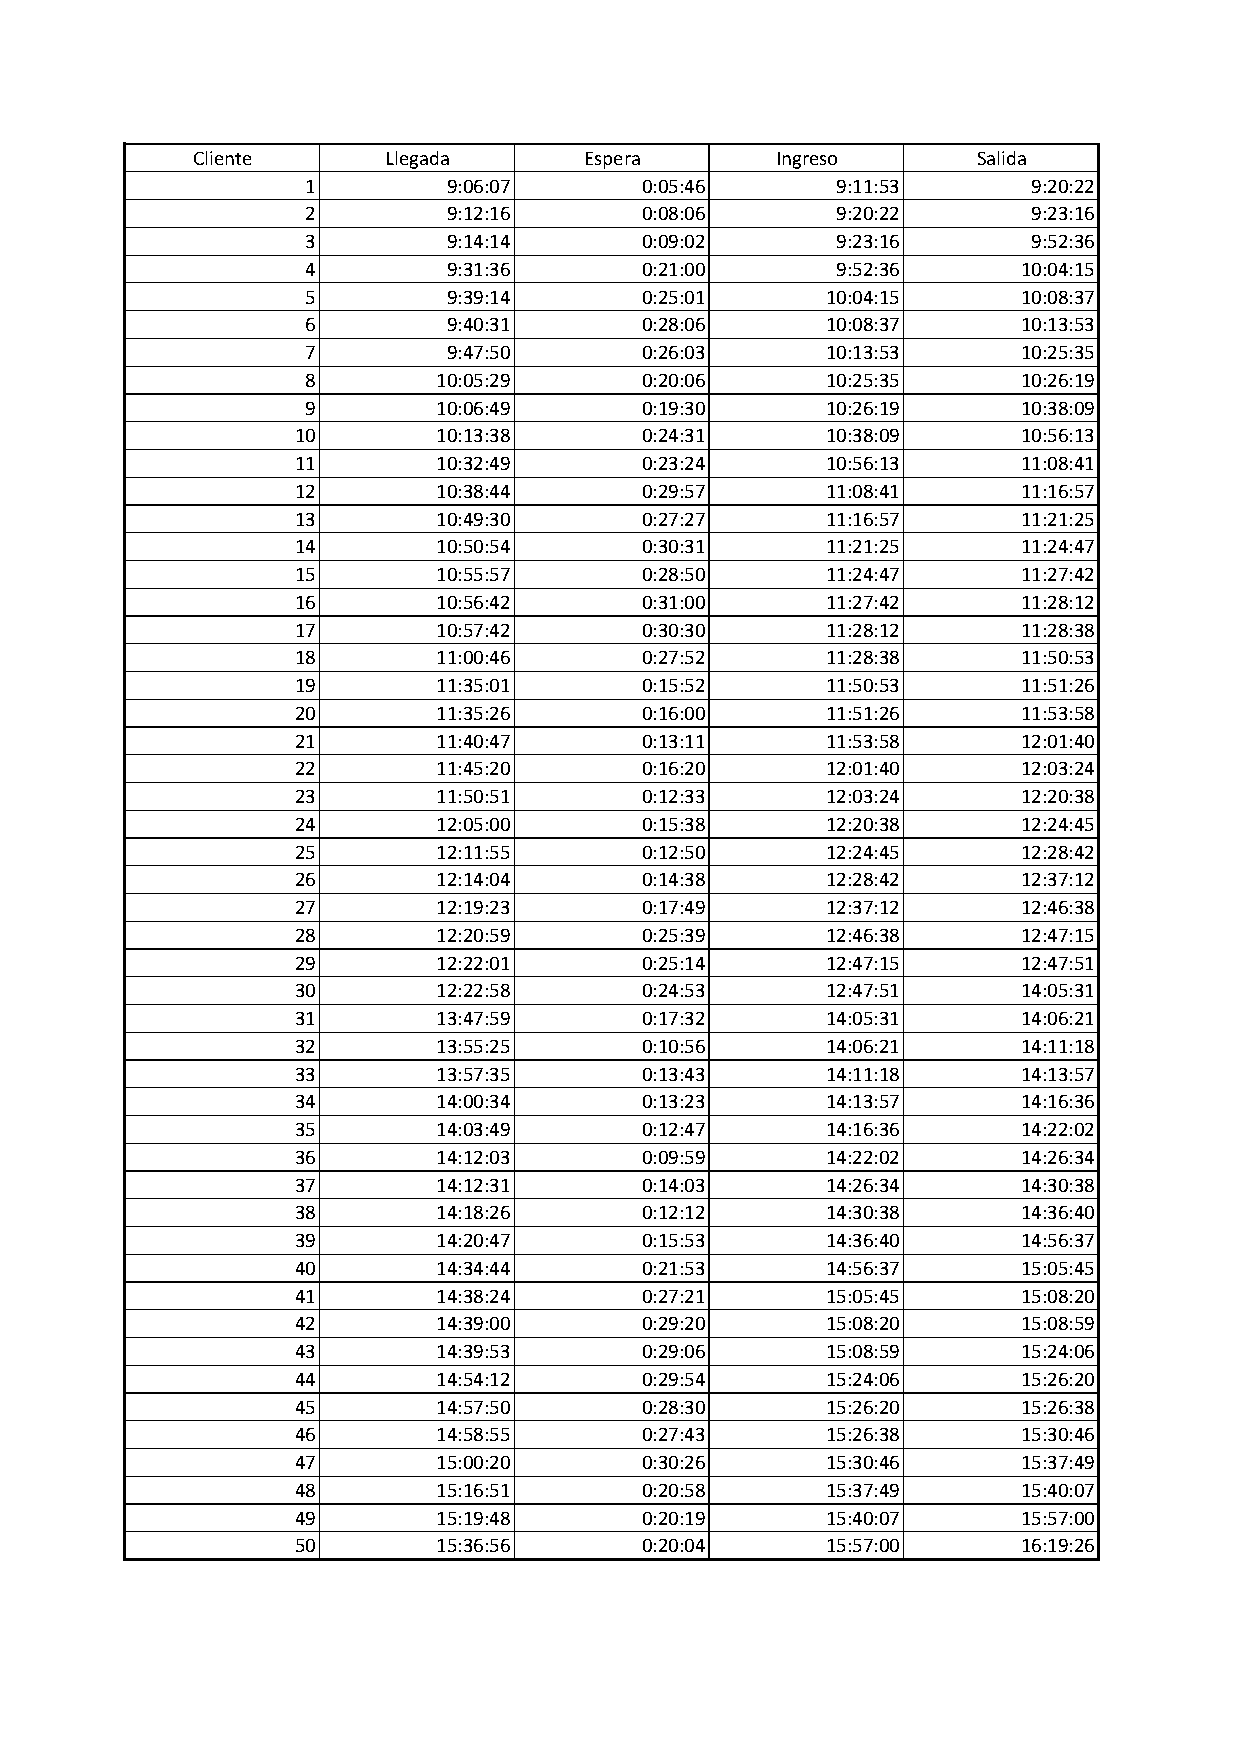
\includepdf[page={1}]{Tabla}
Filtramos los clientes atendidos a partir de dos valores, en este caso, tomaremos la caja 11 y filtraremos acorde a los clientes clasificados como \texttt{CN}. Los datos arrojados por el programa \texttt{QueueSim 1.0.0.0}
\begin{center}
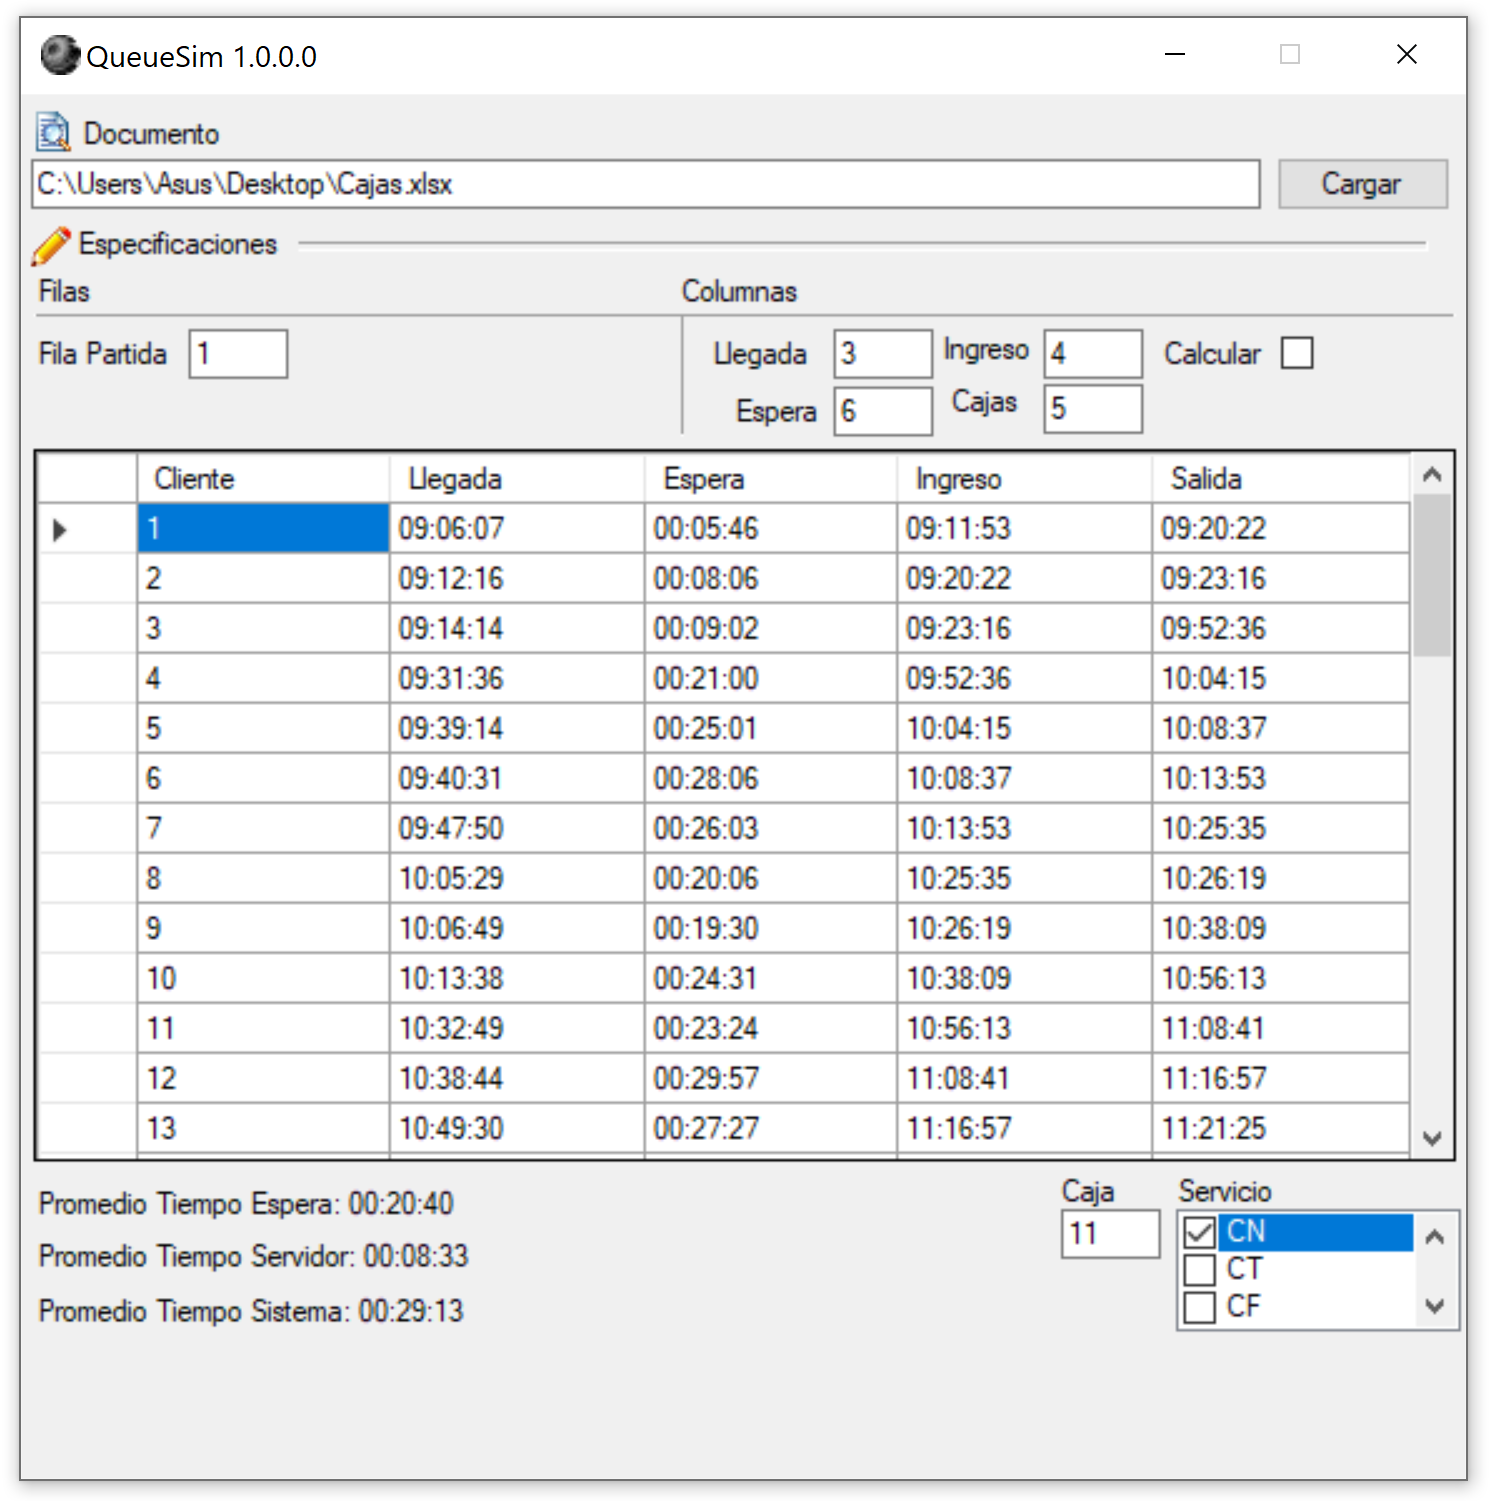
\includegraphics[scale=0.5]{QueueSim_screenshot}
\end{center}
\subsubsection*{Promedios Computados}
$$
\bar{x}=20.6 min. \hspace{1cm} \bar{s}=8.5 min. \hspace{1cm}  \bar{t}=29.21 min.
$$
\subsection*{Computos Método Monte Carlo}


\section*{Conclusiones}
De acuerdo al documento de ``Recopilación de normas para Bancos y Entidades Financieras'' elaborado por la la Autoridad de Supervisión del Sistema Financiero (ASFI), en la Sección 2 (sobre la atención de clientes y usuarios en cajas) en el artículo Nº4 dice lo siguiente:
\begin{fminipage}{\textwidth}
\textbf{Artículo 4$º$ -Tiempo  de  espera  máximo.-} El tiempo  de  espera  máximo  para  que  un  cliente y/o usuario sea atendido en cajas es de treinta (30) minutos. Para efectos del presente reglamento el  tiempo de  espera será  computado  a  partir  de  que  el  cliente  y/o  usuario obtiene  la  ficha  de atención o inicia la fila de espera, hasta el momento en que empieza a ser atendido en caja.
\end{fminipage}
Y de acuerdo a los datos computados, podemos ver que en este caso el tiempo de espera promedio en cola ($\bar{x}$) es 10 minutos inferior a los establecido por la autoridad por lo que podemos ver que en esta sucursal, a partir de una muestra de 50 personas, se esta cumpliendo la regla.
\pagebreak
\section*{Anexos}
\begin{itemize}
\item Recopilación de normas para Bancos y Entidades Financieras, ASFI.\\ \href{https://servdmzw.asfi.gob.bo/circular/Textos/T11.pdf}{\texttt{https://servdmzw.asfi.gob.bo/circular/Textos/T11.pdf}}
\end{itemize}

\end{document}